\documentclass[a4paper,12pt,titlepage]{article}
\usepackage{palatino}
\usepackage{graphicx}
\usepackage{float}
\usepackage{amsmath}
\usepackage{caption}
\usepackage{subcaption}
\usepackage[margin=1.5cm,includefoot]{geometry}
\usepackage[utf8]{inputenc}
\usepackage{hyperref}
\usepackage{url}
\usepackage{listings}
\usepackage{xcolor}
\definecolor{bluekeywords}{rgb}{0.13,0.13,1}
\definecolor{greencomments}{rgb}{0,0.5,0}
\definecolor{redstrings}{rgb}{0.9,0,0}

\usepackage{listings}
\lstset{language=[Sharp]C,
	showspaces=false,
	showtabs=false,
	breaklines=true,
	showstringspaces=false,
	breakatwhitespace=true,
	escapeinside={(*@}{@*)},
	commentstyle=\color{greencomments},
	keywordstyle=\color{bluekeywords}\bfseries,
	stringstyle=\color{redstrings},
	basicstyle=\ttfamily
}

%\lstdefinestyle{sharpc}{language=[Sharp]C, frame = lrtb, rulecolor=\color{blue!80!black}}




\title{\textbf{ \Huge{Integração entre PSoC e Smartphone}}\\}

\author{Victor São Paulo Ruela\\
	Universidade Federal de Minas Gerais}

\date{\today}

\renewcommand*\contentsname{Sumário}


\begin{document}


\maketitle

\tableofcontents
\newpage

\section{Introdução}
	O projeto consiste na integração de dados entre um system-on-ship (PSoC) e um aplicativo Android, utilizando para isso um Web Service na plataforma .NET.
	Através do aplicativo, o usuário consegue visualizar a temperatura do PSoC pressionando um botão. Também foi implementado um cliente Web para consumir o Web Service. Este cliente possui um botão para requisitar a leitura da temperatura do PSoC e a partir dessas leituras, constrói uma tabela contendo todos os valores lidos. Portanto, a seguinte arquitetura de integração foi implementada:
	
	\begin{figure}[h!]
		\centering
		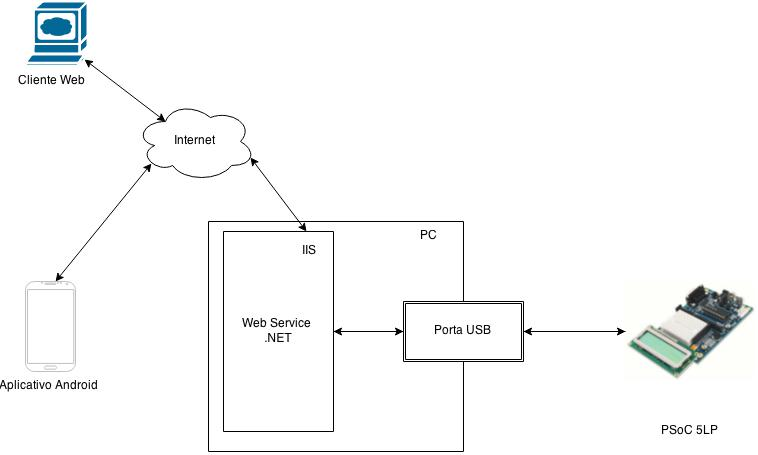
\includegraphics[width=0.7\linewidth]{arquitetura}
		\caption{Arquitetura da integração}
		\label{fig:diagrama}
	\end{figure}
	  
\section{Implementação}
	\subsection{Aplicação do PSoC}
		A aplicação foi feita no PSoC Creator. A criação de uma aplicação para o PSoC é feita através de diagrama de blocos e em C. Inicialmente, colocamos as instâncias dos componentes que serão utilizados em uma página do arquivo \textbf{TopDesig.cysch}, que é o padrão de qualquer projeto no PSoC Cretor. Depois precisamos inicializar e interligar os diversos componentes através das APIs de cada componente, em linguagem C. Para este projeto, foi foram necessários os componentes \textbf{DieTemp} e \textbf{USBUART}. O primeiro permite a leitura da temperatura do PSoC enquanto o segundo habilita o uso da porta USB da placa. Ambos foram usados com a configuração padrão.
			\begin{figure}[h!]
				\centering
				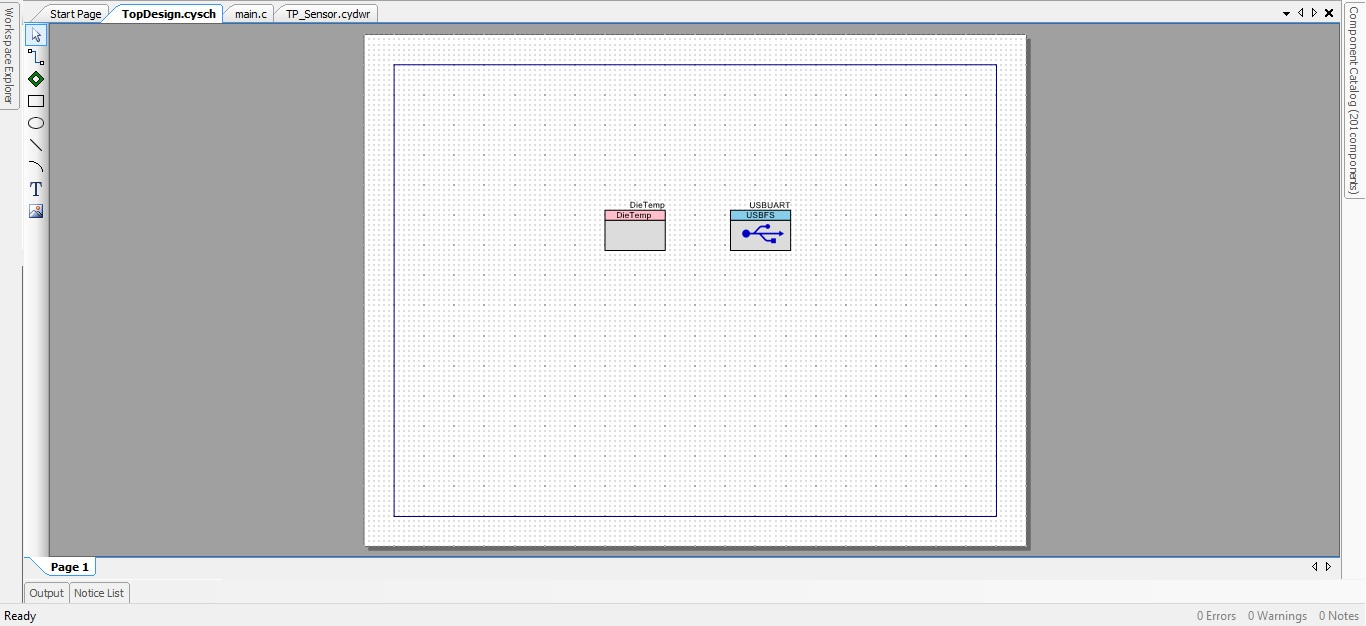
\includegraphics[width=0.8\linewidth]{psoc1}
				\caption{Diagram de blocos no PSoC}
				\label{fig:psoc1}
			\end{figure}
		
		O código em C utiliza as funções da API de cada componente. A lógica de funcionamento da aplicação é bem simples:
			\begin{enumerate}
				\item Inicializar o componente \textbf{USBUART}
				\item Aguardar enumeração da porta USB
				\item Aguardar mensagem de requisiçao de leitura
				\item Obter temperatura através do bloco \textbf{DieTemp}
				\item Enviar para a porta USB				  
			\end{enumerate}
		O PSoC fica em um loop infinito aguardando novas mensagens de requisição de leitura. O bloco USBUART funciona como uma porta serial COM, facilitando a leitura e escrita de dados pela aplicação \textbf{.NET} do Web Service. 
		
			 
	\subsection{Web Service}
		O Web Service está implementado na platforma .NET versão 4.0, usando a linguagem C\#. Ele será publicado em um servidor web local através do \textbf{IIS - Internet Information Services}.Foi necessário realizar uma configuração do roteador: redirecionamento da porta 80 ao endereço de IP local da máquina conectada ao PSoC, para tornar o Web Service visível a todos os computadores e dispositivos conectados à rede. 
		A publicação de Web Service foi facilitada com o uso do \textbf{MS Visual Studio 2012}, o qual possui uma ferramenta muito útil para a publicação de aplicativos Web. Isso reduziu bastante o tempo necessário para desenvolver a aplicação, uma vez que não foram encontrados muitos problemas relacionados à configuração do IIS. O Web Service foi configurado para funcionar com o protocolo SOAP e os métodos  GET e POST do http. 
		
		\subsubsection{Estrutura da aplicação}
			Decidi por implementar o Web Service usando ASMX, porque seu uso ele é mais simples e fácil de configurar, e atendia a todos os requisitos do projeto: uso do HTTP(SOAP) e do IIS. O WCF também poderia ser usado, mas é uma ferramenta mais avançada e poderosa. Como a aplicação desenvolvida é simples, seu uso se mostrou desnecessário.   
			O Web Service fornece dois serviços:
			\paragraph{ReadPSoC}
				Serviço responsável pela comunicação com o PSoC através da porta USB, consumido principalmente pelo aplicativo Android. Inicialmente, ele obtém uma lista de valores de temperatura através da variável Session, que contém os dados de sessão para um determinado usuário. Feito isso, começa a troca de dados propriamente dita:
				\begin{enumerate}
					\item Criação do objeto SerialPort:
								\begin{lstlisting}	
SerialPort s = new SerialPort("COM3", 9600);
								\end{lstlisting}
						  O parâmetro COM3 é o número da porta COM e 9600 é a baudrate da porta, definida na configuração do bloco USBUART.
					\item Abertura da porta serial:
								\begin{lstlisting}	
s.Open();
								\end{lstlisting}
					\item Escrita e leitura na porta serial:
								\begin{lstlisting}	
s.WriteLine("OK");
line = s.ReadLine();								
								\end{lstlisting}
							O dado lido também é adicionado à lista descrita acima, para ficar disponível ao usuário da aplicação Web.
					\item Fechamento da porta serial:
								\begin{lstlisting}	
s.Close();
								\end{lstlisting}
																  
				\end{enumerate}
			As funções acima fazem parte da biblioteca\textbf{System.IO.Ports} do .NET.
			O código possui tratamento de exceções para evitar que a leitura falhe e comprometa a integração do sistema. A principal exceção gerada ocorre quando tentamos ler com o PSoC desconectado do computador. Nesse caso, o Web Service envia a mensagem "Error opening port", indicando a falha. 
			O serviço retorna uma string, contendo a temperatura lida e uma \textit{time stamp} indicando o momento em que a leitura foi feita.
		
			\paragraph{getReadings}
				Serviço usado pela aplicação Web, que será explicada com mais detalhes à frente. Ela retorna uma lista de strings contendo as temperaturas lidas salvas na variável Session do usuário. 
				
		  Ambos os servicos são definidos como \textbf{[WebMethod(EnableSession=true)]}. Esse parâmetro permite salvar e recuperar valores do usuário que está acessando página Web. 
	
	\subsection{Aplcativo Android}
	
	\subsection{Clente Web}
		O cliente Web foi implementado usando Web Forms ASP.NET. A página foi desenvolvida em HTML e contém uma breve descrição de sua funcionalidade, um botão para requisitar a leitura do PSoC e uma tabela mostrando os valores recentemente lidos pelo usuário. Ao requisitar o botão, o seguinte script em C\# é executado:
			\begin{lstlisting}	
 protected void btnRead_Click(object sender, EventArgs e)
 {
	 // Criar instancia do objeto ReadPSoCService
	 ReadPSoCService.Service1SoapClient client =
			 new ReadPSoCService.Service1SoapClient();
 
	 // Realiza leitura do PSoC
	 string result = client.ReadPSoC();
	 // Exibe o resultado na pagina
	 lblResult.Text = result;
 
	 // Associa a variavel com os valores da tabela a lista retornada pelo servico
	 gvReadings.DataSource = client.getReadings();
	 gvReadings.DataBind();
 
	 gvReadings.HeaderRow.Cells[0].Text = "Recent Temperature Readings";
 }
 
 
	 		\end{lstlisting}
			Inicialmente, precisamos adicionar uma referência ao serviço fornecido pelo Web Service ao projeto. Feito isso, criamos uma instância de um objeto representando o serviço acima. Logo, podemos acessar ambos os serviços definidos anteriormente (\textbf{ReadPSoC} e \textbf{getReadings}. \textbf{ReadPOsC} é usado para fazer a leitura do PSoC quando clica-se no botão e \textbf{getReadings} é necessária para montar a tabela com os valores lidos, pois ela acessa a variável contendo os dados de sessão do ususário. 
			 
		
\section{Resultados}
	\subsection{Cliente Web}
	O cliente Web foi testado em diversos computadores na rede local e seu funcionamento foi como o esperado em todos os casos. A página web foi acessada de um computador com sistema operacional Windows, outro com iOS e de smartphones, funcionando corretamente em todos. 
	
	
	\subsection{Aplicativo Android}
	O aplicativo Android foi testado no emulador de dispositivos Android e em um Nexus 4. Ambos funcionaram perfeitamente.
	
		\begin{figure}[h!]
			\centering
			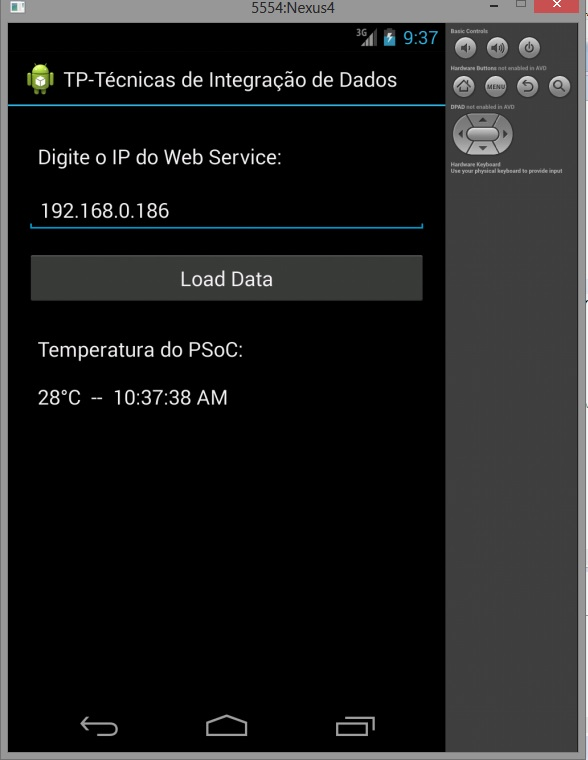
\includegraphics[width=0.4\linewidth]{appemulador}
			\caption{Screenshot do emulador de Dispositivos Android}
			\label{fig:emulador}
		\end{figure}
		

\section{Conclusão}

\end{document}